\documentclass{standalone}
\usepackage{tikz}
\usetikzlibrary{arrows, positioning, calc}
\usepackage{graphicx}
\begin{document}
\begin{tikzpicture}[node distance=5cm, >=stealth, transform shape, scale=2]
  \node (noise) at (0,0) {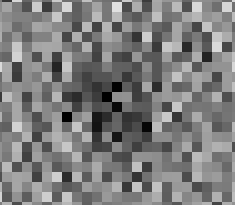
\includegraphics[height=6cm]{nuc12syg1-noise.png}}; 
  \node[yshift=0.1cm] at (noise.north) {\sf Original data};
  \node[right=of noise] (gauss) {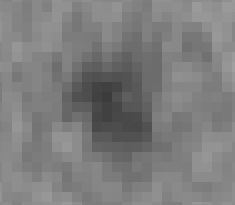
\includegraphics[height=6cm]{nuc12syg1-gauss.png}}; 
  \draw[->, very thick] (noise) -- node[above] {\sf 2d gauss smoothing (radius=1)} (gauss);
  %\node[right=of gauss, xshift=-3cm] (onepixel)  {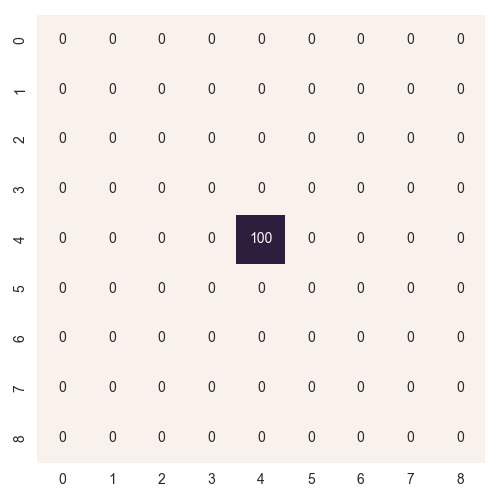
\includegraphics[height=6cm]{./before_gauss.png}}; 
  %\node[right=of onepixel] (smoth) {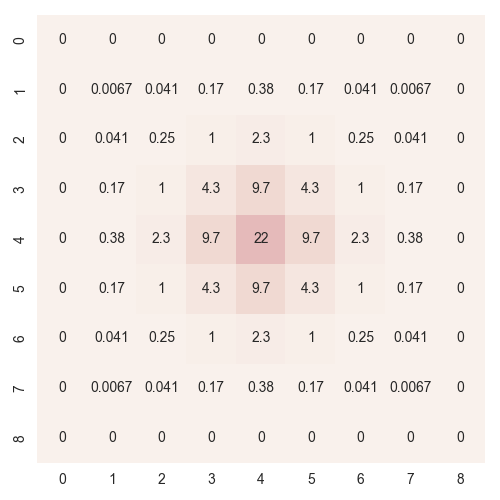
\includegraphics[height=6cm]{./after_gauss.png}}; 
  %\draw[->, very thick] (onepixel) -- node[above] {\sf 2d gauss smoothing (radius=1)} (smoth);
  %\node at ($(onepixel.north)!.5!(smoth.north)$) {\sf Gauss smoothing example}; 
  \node (noise) at (0,-7cm) {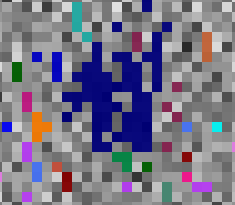
\includegraphics[height=6cm]{./nuc12syg1-label.png}}; 
  \node[yshift=0.1cm] at (noise.north) {\sf Labeled data};
  \node[right=of noise] (gauss) {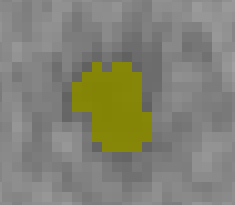
\includegraphics[height=6cm]{./nuc12syg1-gauss-label.png}}; 
  \draw[->, very thick] (noise) -- node[above] {\sf 2d gauss smoothing (radius=1)} (gauss);
  %\node[right=of gauss, xshift=-3cm] (onepixel)  {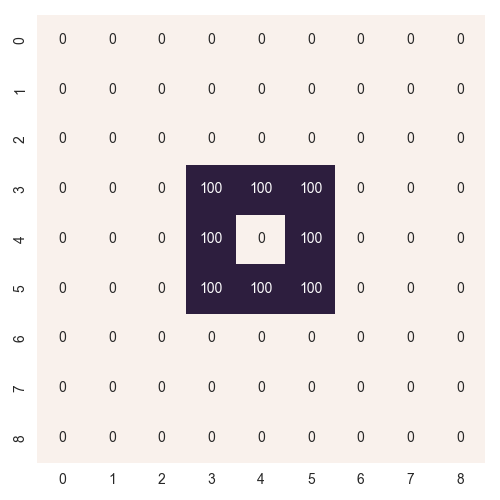
\includegraphics[height=6cm]{./before_gauss_big.png}}; 
  %\node[right=of onepixel] (smoth) {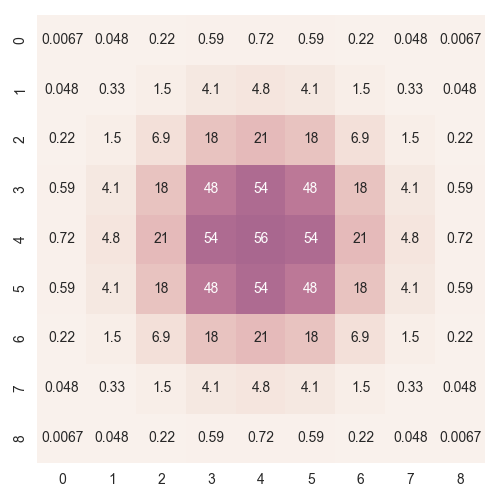
\includegraphics[height=6cm]{./after_gauss_big.png}}; 
  %\draw[->, very thick] (onepixel) -- node[above] {\sf 2d gauss smoothing (radius=1)} (smoth);
\end{tikzpicture}
\end{document}
